

\documentclass[12pt]{article} 
\usepackage{todonotes}
\usepackage{graphicx}
\usepackage{grffile}
\usepackage{algorithm}
\usepackage[noend]{algpseudocode}
\usepackage{float}
\usepackage[font=footnotesize,labelfont=bf]{caption}
\usepackage[left=0.8in, right=0.8in, top=0.9in, bottom=1in]{geometry}
\usepackage{hyperref} 
%\usepackage{caption}
\graphicspath{ {images/} }


\title{ \textbf {\vspace{0.1cm}\Huge Pipeline with load balancing\\ \vspace{0.3cm}}
 Final Project for the SPM course \vspace{0.5cm}\\} 

\date{\vspace{1.0cm}}

\author{ \Large Francesco Balzano \vspace{0.3cm}\\ 
%Matricola 541533 \vspace{0.5cm}\\
\Large Master Degree in Computer Science and Networking \vspace{0.4cm} \\
\Large A.Y. 2017-2018 
}


\begin{document}
  \pagenumbering{gobble}
  \maketitle
  %\newpage
  \noindent\rule{18cm}{0.4pt}
  \tableofcontents
  \newpage
  \pagenumbering{arabic}

\clearpage
\setcounter{page}{2}
  
\section{Design and Implementation choices}

\subsection{Design} 
I designed a pipeline as a handler for a vector of stages. It takes care to start the execution of all the stages and to await for their termination. Each stage encapsulates a user-defined function and runs it in a separate thread of execution. Each stage takes its tasks from an input buffer and puts the results in an output buffer. Each buffer has limited size and has to guarantee that the tasks are picked with the same order in which they were put in the buffer.

\subsubsection{Pipeline}
A pipeline receives a list of stages and a list of tasks and:
\begin{itemize}
\item builds the chain, ensuring that stage $i$ outputs the results to the input buffer of stage \textit{i+1};
\item sends the received tasks to the first stage, actually starting the chain of computations;
\item when the tasks are exhausted, sends a special task to the first stage to propagate the termination message, and awaits that all the stages terminate the execution.
\end{itemize}
In the mean time a separate thread of execution monitors the execution times of each stage of the pipeline and, for each stage, makes the average of the times. The collapsing of two consecutive stages may be triggered after a certain number of execution times has been measured for each stage. So let's suppose we are in this situation, and let $i$ be the index of the $i^{th}$ stage and $slowest$ the index of the slowest stage: if it exists some $i$ such that: \[ avg\_time_{i} + avg\_time_{i+1} < avg\_time_{slowest} \] then the stage $i$ and the stage $i+1$ are collapsed into a single sequential stage. I decided that collapsing actually means that:
\begin{itemize}
\item Stage $i$ stops its computation until stage $i+1$ terminates and informs stage $i+1$ that it has to be collapsed; 
\item stage $i+1$ makes its computation on the remaining tasks (the ones already in its input buffer) and then terminates its execution;
\item stage $i$ resumes its computation: from now on it will run the computations of stage $i+1$ too.
\end{itemize}
Since in the project text it was requested only the merge of two consecutive stages, I decided that a stage can merge the adjacent stage in the pipeline, but not more than one. In other words, a stage can at most run its computation and the next stage's one. 

\subsubsection{Stage}
A stage picks the tasks from an input buffer, applies a user-defined function to each of them and puts the results to an output buffer. It also measures the time that each computation takes. This measure does not take into account the time spent to pick an item from the input buffer or the time spent to put an item into the output buffer. The reason is that a stage could take a lot of time to pick an item because the input buffer is empty, but this may be due to a previous stage which is slow at producing tasks. So it is only measured the time that each stage takes to compute the assigned function. 

\subsubsection{Buffer}
The data structure that implements the buffer has the following features:
\begin{itemize}
\item thread-safe, because it is accessed concurrently by the stage $i$ to put a new task and by the stage $i+1$ to pop a task 
\item ordered, because stage $i+1$ must pick the tasks in the very same order in which they were put by stage $i$
\item priority, because the ``collapse'' message must get the highest priority, so that is immediately picked by the receiving stage although there are other messages in the buffer
\end{itemize}
I decided that the priority of each message inserted in the buffer is explicitly assigned by the entity that puts a new message in the buffer, rather than by the buffer itself. In my opinion this gives greater flexibility, and semplifies the responsabilities of the buffer which has only to guarantee that the provided order is maintained.

\subsection{Implementation}
In the following paragraphs I describe, class by class, the main implementation choices. Each class is actually a struct, so their methods and members are completely visible.

\subsubsection{Pipe.hpp}
A Pipe is parametrized with the input type of its first Stage, \texttt{Tin}, and with the output type of its last Stage, \texttt{Tout}. \\
The constructor of a Pipe takes a list of Stages and builds the chain by invoking the method \texttt{add\_next()} of class Stage. \\
To start the computation, the caller must call the method \texttt{run(list<Tin>\&\& input)}, providing a list of tasks as input. This results in the invocation of \texttt{run\_manager()} in a separate thread of execution, in the repeated invocation of \texttt{monitor\_times()} until a termination condition satisfied, and finally in the wait that the thread running \texttt{run\_manager()} ends its execution. \\
The method \texttt{run\_manager()} starts the execution of each Stage in a separate thread, puts all the received tasks in the input buffer of the first Stage (possibly blocking if the buffer gets full), sends the special termination message \texttt{nullptr} to the first Stage when the tasks are exhausted and waits for the termination of each Stage. It also sets the termination condition after the termination message is sent. The reason why the termination condition is put here and not after all the stages ended their execution is that otherwise the monitoring of times could continue even after some stages ended their computations. Since the method \texttt{monitor\_times()} is responsible for triggering the collapse of stages, this could end up in collapsing a stage which has already ended its computations, which has no sense. \\
The method \texttt{monitor\_times()} takes care of monitoring the execution times and triggering the collapse of the Stages. It consists of three phases: initialization, monitoring and collapse. The last two phases are repeated until the termination condition is met.
\begin{itemize}
\item initialization: three vectors \texttt{count}, \texttt{avg} and \texttt{measures} are initialized. \texttt{count[i]} gives the number of execution times measured for Stage $i$; \texttt{avg[i]} gives the current average execution time of Stage $i$; \texttt{measures[i]} holds a priority queue that contains the last measures, the ones from which \texttt{avg[i]} has been computed. 
\item monitoring: all the Stages are scanned and their execution times are read. The same execution time is never counted twice because after it is read, it is immediately set to zero. Then for each Stage $i$ with a fresh execution time, a measure is created and inserted in the priority queue \texttt{measures[i]}. A measure is a pair in which the first element is the execution time and the second element is the number of that execution. This number is used to order the measures: indeed if the number of measures taken from the beginning of the monitoring for Stage $i$ exceeds the threshold \texttt{num\_samples}, then the oldest measure in the priority queue is popped. Each priority queue keeps only the last measures and at steady state it keeps exactly \texttt{num\_samples} measures. The measures in the priority queue \texttt{measures[i]} are the same used to compute the average execution time \texttt{avg[i]}. This average is computed incrementally every time a new measure is taken. 
\item collapse: this phase is run only if the execution times have been measured at least \texttt{num\_samples} times for each Stage. In this case if it exist two Stages such that the sum of their average execution times is smaller than the execution time of the slowest Stage, then they are collapsed into a single sequential stage. Two stages can be collapsed only if both of them have not been already collapsed by another Stage and did not collapse any Stage.
\end{itemize}

\subsubsection{Stage.hpp}
The abstract class IStage is the interface for a Stage.
A Stage is parametrized with the type of its input tasks, \texttt{Tin}, and with the type of its results, \texttt{Tout}. \\
The constructor of a Stage takes as parameter the function that the Stage has to apply to each input task. \\
To run a task the caller must invoke the method \texttt{run()}, which executes \texttt{run\_thread()} in a separate thread of execution and assigns the newly created thread to a member variable. This way it is possible to wait for thread completion in a second moment. \\
The method \texttt{run\_thread()} runs the assigned function on the input tasks until a termination condition is met. Anyway, the execution of such function is stopped if the current Stage is collapsing the next Stage: in this case indeed we have to wait that the next Stage finishes all its tasks and terminates its execution before producing new results. The execution of the function ends when \texttt{nullptr} is received in input. At this point a finalization is performed: if the Stage is terminated because it has received the last task of the stream (\texttt{collapsed $\neq$ -1}), then it propagates the termination message and if the next Stage has been collapsed, this Stage runs also its function. If instead this Stage is terminated because it has been collapsed, it runs its function on every remaining task and then terminates without propagating the termination message. \\
The method \texttt{set\_input()} is used to insert a new task in the input buffer of the receiving Stage. This method is also responsible for updating the count of the number of tasks received in input by the Stage. This allows to pick tasks from the input buffer in correct order. \\
The method \texttt{collapse\_next\_stage()} is responsible for collapsing the next Stage. Collapsing basically means that the next Stage executes the computation on the remaining tasks and then the corresponding thread terminates. A boolean variable \texttt{collapsing} is used to ensure that this Stage will not produce any new task in output while it is collapsing the next Stage.

\subsubsection{TSOHeap.hpp}
This class implements the buffer. The name stands for ``Thread-Safe Ordered Heap''. \\
It is a heap because the main data structure that it wraps is a priority queue, that is basically a heap. As already said, the heap is needed because we want both to keep the ordering of the tasks and to give the highest priority to special tasks that indicate imminent collapse. This is achieved by inserting in the heap pairs where the first element is the actual task and the second element is an integer \texttt{id} that states the order in which tasks have to be extracted from the heap. The struct ``Comparator'' is a functor passed to the heap to enforce the priority that we want. Since the value of \texttt{id} is increasing with the number of tasks that we receive, the simple ordering that we impose is that at any time the pair extracted from the heap is the one with smallest \texttt{id}. This is the reason why the heap is called ordered. Special tasks are assigned the highest priority by simply pairing them with the smallest possible integer. \\
Finally it is thread-safe because the two methods  \texttt{pop()} and \texttt{push()} are both thread-safe. A thread that invokes the \texttt{push()} method to insert a new pair in the heap waits if the heap is full, while a thread that invoks the \texttt{pop()} method to pick the pair with smallest \texttt{id} waits if the heap is empty. Both waits are active waits, realized with the use of atomic variables, so that a thread is not descheduled from processor when waiting. For the remaining part of these methods I used a mutex to guarantee mutual exclusion in the access to the priority queue.
  

\begin{figure}
\centering
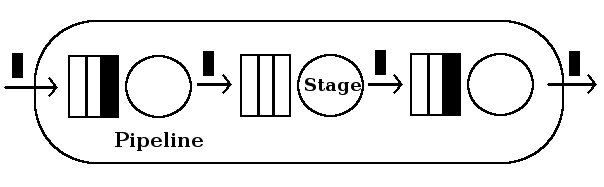
\includegraphics[scale=0.43]{Pipe}
\caption{The pipeline is a chain of sequential stages. There is a buffer of limited size between each pair of consecutive stages.}
\label{fig:pipe}
\end{figure}     

\section{Manual}
    

\section{Results}

\subsection{Limitations}





\end{document}
